\chapter{Sistemas dinámicos}

\section{Generalidades}

En ingeniería estructural, un sistema se refiere al conjunto de elementos estructurales interconectados que trabajan en conjunto para resistir cargas y garantizar la estabilidad y seguridad de una construcción. En particular, un sistema dinámico es una estructura cuya respuesta varía en el tiempo ante cargas cambiantes, como sismos, viento, impactos o transito.

Al estudiar sistemas dinámicos es fundamental distinguir entre el sistema físico y el modelo matemático. El sistema físico es la estructura real, con sus materiales, geometría y condiciones de carga, sujeta a imperfecciones y a interacciones complejas con el entorno. En cambio, el modelo matemático es una representación simplificada que traduce ese comportamiento en ecuaciones, permitiendo predecir su respuesta bajo distintas condiciones.

Estos modelos matemáticos se construyen a partir de principios fundamentales, es decir, de las leyes físicas que gobiernan la mecánica estructural. Entre ellas destacan la cinemática y compatibilidad geométrica, ecuaciones de balance (Newton, Lagrange, etc.), relaciones constitutivas de los materiales, y la geometería y condiciones de contorno e iniciales del sistema físico. A partir de estos principios, se generan modelos matemáticas que representan de forma coherente el comportamiento de la estructura, aunque siempre con ciertas simplificaciones necesarias para el análisis.

Los sistemas sistemas dinámicos pueden ser representados gráficamente por diagramas de bloques:

\begin{figure}[H]
    \centering
    
\includegraphics[scale=0.7]{sistema.png}
    \caption{Representación de un sistema dinámico}
\end{figure}

Principales razones para construir modelos matemáticos de sistemas dinámicos:

\begin{enumerate}
    \item Análisis
    \item Diseño
    \item Control y monitoreo
\end{enumerate}

\section{Tipos de sistemas}

\subsection{Estáticos vs Dinámicos}

\begin{itemize}
    \item Sistema Estático: respuesta solo depende de la excitación actual (independiente del tiempo).
    \begin{figure}[H]
    \centering
    
\includegraphics[scale=0.7]{estatico.png}
    \end{figure}
    
    \item Sistema Dinámico: respuesta actual depende de la excitación actual y de la ``historia'' de la respuesta.
    \begin{figure}[H]
    \centering
    
\includegraphics[scale=0.7]{dinamico.png}
    \end{figure}
    \par Si la respuesta del sistema dinámico está basada en la excitación actual y pasada, entonces el sistema se conoce como \textcolor{red}{causal} (todos los sistemas físicos).\\
    \par Si la respuesta del sistema dinámico está basada en excitación actual, pasada y \textcolor{ForestGreen}{futura}, entonces el sistema es \textcolor{red}{anticausal} (solo aplicable en sistemas teóricos \emph{offline}, por ejemplo, en procesamiento digital de señales).
\end{itemize}

\subsection{Univariado vs Multivariado}
\begin{itemize}
    \item SISO: Single Input, Single Output.
    \begin{figure}[H]
    \centering
    
\includegraphics[scale=0.7]{SISO.png}
    \end{figure}
    \begin{itemize}
        \item $u \in \mathbb{R}$: entrada escalar
        \item $y \in \mathbb{R}$: respuesta escalar
        % \item $f(u)=y$: función escalar
    \end{itemize}
    
    \item SIMO: Single Input, Multi Output.
    \begin{figure}[H]
    \centering
    
\includegraphics[scale=0.7]{SIMO.png}
    \end{figure}
    \begin{itemize}
        \item $u \in \mathbb{R}$: entrada escalar
        \item $y \in \mathbb{R}^m$: respuesta vectorial
    \end{itemize}
    
    \item MISO: Multi Input, Simple Output.
    \begin{figure}[h]
    \centering
    
\includegraphics[scale=0.7]{MISO.png}
    \end{figure}
    \begin{itemize}
        \item $u \in \mathbb{R}^n$: entrada vectorial
        \item $y \in \mathbb{R}$: respuesta escalar
    \end{itemize}
    
    \item MIMO: Multi Input, Multi Output.
    \begin{figure}[H]
    \centering
    
\includegraphics[scale=0.7]{MIMO.png}
    \end{figure}
    \begin{itemize}
        \item $u \in \mathbb{R}^n$: entrada vectorial
        \item $y \in \mathbb{R}^m$: respuesta vectorial
    \end{itemize}
\end{itemize}

\subsection{Lineal vs Nolineal}

\begin{itemize}
    \item Un \emph{sistema lineal} es tal que cumple con el \emph{principio de superposición}.
    
    \begin{itemize}
        \item Aditividad: Si $u_1 \rightarrow y_1$, $u_2 \rightarrow y_2$, entonces: $u = u_1 + u_2 \rightarrow y = y_1 + y_2$
        \item Homogeneidad/Proporcionalidad: Si $u \rightarrow y$, entoncecs ${\alpha}u \rightarrow {\alpha}y$.
    \end{itemize}
    \item De no cumplir con las propiedades del sistema lineal, entonces el sistema es \emph{nolineal}.
\end{itemize}

\par \underline{Ejemplo}: resorte nolineal.\\

\begin{figure}[H]
    \centering
    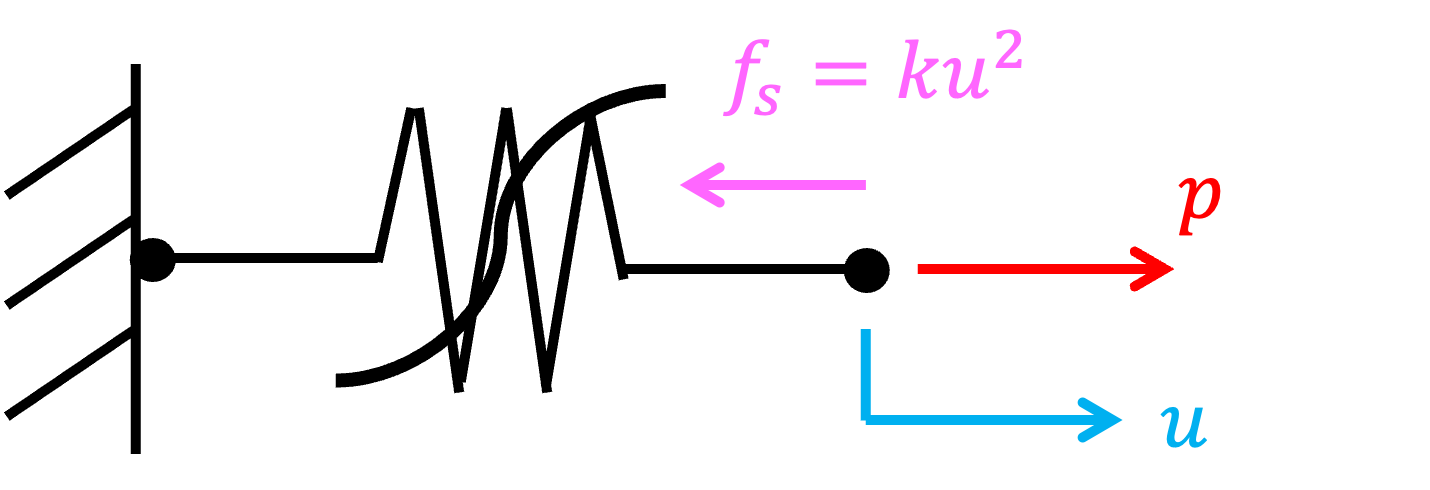
\includegraphics[scale=0.7]{Figuras/resortenolineal.png}
    \caption{Resorte nolineal}
\end{figure}

Se tiene que: 

\begin{align*}
    f_s &= ku^2 \\
    p_1 = k u_1^2 &\rightarrow u_1 = \sqrt{\frac{p_1}{k}}\\  
    p_2 = k u_2^2 &\rightarrow u_2 = \sqrt{\frac{p_2}{k}}\\
\end{align*}

La pregunta es, ¿Se cumple el principio de superposición?

\begin{align*}
    p_1+p_2 &\xrightarrow{?} u_1+u_2
\end{align*}

La respuesta es {no}, ya que:

%\begin{align*}
%    f_s &= k(u_1+u_2)^2 \\
%    p_1 + p_2 & = ku_1^2+ku_2^2+2ku_1u_2\\
%    p_1 + p_2 &\neq p_1 + p_2 + \textcolor{red}{2ku_1u_2}
%\end{align*}

\begin{align*}
    p_1 + p_2 &= k(u_*)^2 \\
    u_* &= \sqrt{\frac{p_1 +p_2}{k}} \neq \sqrt{\frac{p_1}{k}} + \sqrt{\frac{p_2}{k}}
\end{align*}

\subsection{Invariante tiempo vs variante tiempo}

\begin{itemize}

    \item Sistema invariantes en el tiempo (\emph{time invariant}) $\longrightarrow$ parámetros del modelo son constantes en el tiempo.\\
    
    \underline{Ejemplo}: Sistemas de 1GDL (Figura \ref{f:invariante}),  con masa, rigidez y amortiguamiento constante son LTI (\emph{linear time invariant}).
    
    \begin{figure}[h]
        \centering
        
\includegraphics[scale=0.7]{invariante.png}
        \caption{Sistema LTI (\emph{linear time invariant})}
        \label{f:invariante}
    \end{figure}
    
    \item Sistema variante en el tiempo (\emph{time variant}) $\longrightarrow$ parámetros del modelo varían en el tiempo.\\
    
    \underline{Ejemplo}: Puentes con masa movil (Figura \ref{f:movingmass}), por ejemplo por el transito de un vehículo pesado (la masa del sistema varía). En este caso el sistema dinámico es LTV (\emph{linear time variant}).

    \begin{figure}[h]
        \centering
        \includegraphics[width=0.5\textwidth]{movingmass.png}
        \caption{Sistema LTV (\emph{linear time variant})}
        \label{f:movingmass}
    \end{figure}
    
\end{itemize}

\subsection{Determinístico vs Estocástico}

Si el input del sistema es conocido (y el sistema no incorpora incertidumbre), entonces el output será predecible $\longrightarrow$ \textcolor{red}{Determinístico} \\ 

\underline{Ejemplo}: Simular múltiples veces el mismo registro (input) sobre el mismo edifico (sistema), se obtienen siempre las mismas respuestas (output). \\

Si el input del sistema posee incertidumbre (y/o el sistema incorpora incertidumbre), entonces el output también tiene incertidumbre y no es predecible $\longrightarrow$ \textcolor{red}{Estocástico} \\

\underline{Ejemplo}: Simular peatones diferentes (input con incertidumbre en masa del peatón, velocidad al caminar y frecuencia de pasos) sobre un mismo puente (sistema), se obtendrán respuestas diferentes (outputs)\\

% María: Si los parámetros del modelo son conocidos $\longrightarrow$ \textcolor{red}{Determinístico}.\\
% María: Pero, si existe incertidumbre en alguno de los parámetros, o si no se puede predecir de manera precisa la respuesta del sistema $\longrightarrow$ \textcolor{red}{Estocástico}.

\subsection{Continuo vs Discreto}
\begin{itemize}
    \item Sistema Continuo: entrada y salida son función del tiempo.
    \begin{figure}[H]
    \centering
    
\includegraphics[scale=0.7]{continuo.png}
    \end{figure}
    \item Sistema Discreto: señales han sido discretizadas en el tiempo.\\
    % Ale: Reemplazar el ejemplo por siguiente línea:
    % Ejemplo: Registro de aceleraciones?
    \underline{Ejemplo}: Interés de una cuenta bancaria.
    \begin{align*}
        y(k+1)=(1+r)y(k) \longrightarrow \text{Ecuación de diferencias finitas}
    \end{align*}
    \begin{itemize}
        \item $y(k+1)$: balance cuenta año $k+1$
        \item $r$: interés compuesto anual
        \item $y(k)$: balance cuenta año $k$
    \end{itemize}
\end{itemize}

Las señales de los sistemas físicos son continuas, pero que al momento de ser \emph{observadas} por dispositivos digitales, estas señales se discretizan en función del tiempo.

\begin{figure}[h]
    \centering
    
\includegraphics[scale=0.7]{time_sampling.png}
    \end{figure}

\section{Respuesta de sistemas LTI en tiempo continuo}
LTI: Linear, Time-Invariant.

\begin{figure}[H]
    \centering
    
\includegraphics[scale=0.7]{sistemayu.png}
\end{figure}

Los sistemas LTI, son aquellos cuyas propiedades y parámetros no varían en el tiempo, es decir, que los coeficientes de las ecuaciones diferenciales de los modelos matemáticos de los sistemas dinámicos son constantes en el tiempo $a_i=cte$.
\begin{align*}
    \frac{d^ny}{dt^n}+a_{n-1}\frac{d^{n-1}y}{dt^{n-1}}+...+a_2\frac{d^2y}{dt^2}+a_1\frac{dy}{dt}+a_0y=u(t)
\end{align*}
\begin{itemize}
    \item $u(t)$: excitación
    \item $y(t)$: respuesta
    \item $a_i$: coeficientes
\end{itemize}
Dada una excitación $u(t)$, la respuesta se obtiene al resolver la ecuación diferencial:
\begin{align*}
    y(t)=y_H(t)+y_p(t)
\end{align*}
\begin{itemize}
    \item $y_H(t)$ es la \textcolor{red}{respuesta homogénea} (para $u(t)=0$, con condiciones iniciales)
    \item $y_p(t)$ es la \textcolor{red}{respuesta particular} (para $u(t)\neq0$)
\end{itemize}

\section{Modelos de sistemas dinámicos}

Existen diversas formas de modelar un sistema dinámico.

\begin{figure}[H]
    \centering
    
\includegraphics[scale=0.8]{modelos.png}
    \caption{Relaciones entre distintas representaciones de modelos de sistemas dinámicos.}
\end{figure}

\section{Función de transferencia de un sistema de 1GDL}
\begin{figure}[H]
\centering

\includegraphics[scale=0.7]{edm.png}
\end{figure}
\underline{Problema}: Dada la EDM de un sistema estructural 1GDL, determinar su función de transferencia $H(s)$\\ 
\par Notación: 
\begin{align*}
    U(s) &= \mathcal{L}\{u(t)\}~: \text{respuesta (dominio complejo)}\\
    F(s) &= \mathcal{L}\{f(t)\} ~: \text{input (dominio complejo)}
\end{align*}

Asumiendo reposo: $u(0)=\dot{u}(0)=0$

\begin{align*}
    m\ddot{u}+c\dot{u}+ku &= f(t) ~/\color{red}{\mathcal{L}\{\cdot\}}\\
    m\mathcal{L}\{\ddot{u}\}+c\mathcal{L}\{\dot{u}\}+k\mathcal{L}\{u\} &= \mathcal{L}\{f\}\\
    ms^2U(s)+csU(s)+kU(s) &= F(s)\\
    (ms^2+cs+k)U(s) &= F(s)
\end{align*}
\begin{align*}
    \Longrightarrow H(s) = \frac{U(s)}{F(s)}&=\frac{1}{ms^2+cs+k} ~\text{: TF del sistema de 1GDL}
\end{align*}

Aparte: Dada la entrada $F(s)$ y la TF $H(s)$, la salida es $U(s) = H(s)F(s)$
\begin{figure}[H]
\centering

\includegraphics[scale=0.7]{hs.png}
\end{figure}

Desde la TF del sistema:
\begin{align*}
    H(s) &= \frac{1}{ms^2+cs+k} ~\color{red}{\frac{1/m}{1/m}}\\
    &= \frac{1/m}{s^2+2\xi\omega_ns+\omega_n^2}
\end{align*}
\begin{itemize}
    \item $\xi$: razón de amortiguamiento
    \item $\omega_n$: frecuencia natural
\end{itemize}

¿Cómo se obtienen los polos? $\Longrightarrow$ Calcular las raíces del polinomio del denominador:
\begin{align*}
    s^2+2\xi\omega_ns+\omega_n^2=0 ~\text{: Ecuación característica}
\end{align*}
\begin{align*}
     s_{1,2}=-\xi\omega_n\pm\omega_n\sqrt{1-\xi^2}j\\
     s_{1,2}=-\xi\omega_n\pm\omega_dj ~\text{: Polos del sistema de 1GDL}
\end{align*}

¿Es estable? $\Longrightarrow$ Depende del valor de $\xi$:
\begin{itemize}
    \item $\xi>0, ~ Re(s_{1,2}<0\Longrightarrow$ Estable asintóticamente
    \item $\xi<0, ~ Re(s_{1,2}>0\Longrightarrow$ Inestable
    \item $\xi=0, ~ Re(s_{1,2}=0\Longrightarrow$ ``Estable''
\end{itemize}

Además, el sistema oscila sí y solo si $\omega_d>0\Longrightarrow \omega_n>0$: propiedad del sistema dinámico.\\
Si $\xi>0, ~ \omega_n>0$:
\begin{figure}[H]
\centering

\includegraphics[scale=0.6]{estabilidad.png}
\end{figure}

% La Función de Respuesta en Frecuencia se obtiene a través de aplicar la transformada de Fourier:
%\begin{align*}
%    H(\omega)=\mathcal{F}\{h(t)\}
%\end{align*}

Notar que el FRF se puede obtener al reemplazar $s=j\omega$ en la TF:
\begin{align*}
    H(\omega)=H(s)\bigg|_{s=j\omega}
\end{align*}

\underline{Ejemplo}: Sistema de 1GDL
\begin{align*}
    \text{EOM: }~m\ddot{u}+c\dot{u}+ku=f(t)
\end{align*}
\begin{align*}
    \Longrightarrow \text{TF: }&~ H(s)=\frac{1}{ms^2+cs+k}=\frac{1/m}{s^2+(c/m)s+k/m}\\
    \Longrightarrow \text{FRF: }&~ H(\omega)=H(s)\bigg|_{s=j\omega}=\frac{1}{(k=m\omega^2)+j\omega c}
\end{align*}
\begin{align*}
    H(\omega)=\frac{1}{(j\omega-\lambda_1)(j\omega-\lambda_1^*)}
\end{align*}
\begin{itemize}
    \item $\{\}^*$: conjugado del número complejo
\end{itemize}
\begin{align*}
    \lambda_1, \lambda_1^*=-\xi\omega_n\pm\omega_n\sqrt{1-\xi^2}~\text{: polos del sistema}
\end{align*}

\section{Función de transferencia de un sistema de MGDL}
La TF de un sistema dinámico de MGDL se obtiene aplicando la transformada de Laplace a la EDM:

\begin{align*}
    \tenq{M}\tend{\ddot{u}}(t)+\tenq{C}\tend{\dot{u}}(t)+\tenq{K}\tend{u}(t)&=\tend{F}(t) ~/\mathcal{L}\{\cdot\}\\
    \Longrightarrow s^2\tenq{M}\tend{U}(s) + s\tenq{C}\tend{U}(s) +\tenq{K}\tend{U}(s) &= \tend{F}(s)\\
    \Longrightarrow\left[s^2\tenq{M}+s\tenq{C}+\tenq{K} \right]\tend{U}(s)&=\tend{F}(s) \\
    \Longrightarrow \tenq{H}(s) = \frac{\tenq{U}(s)}{\tenq{F}(s)} = =\left[s^2\tenq{M}+s\tenq{C}+\tenq{K} \right]^{-1} 
\end{align*}

Donde 
\begin{align*}
    \tend{F}(s) &= \mathcal{L}\{\tend{f}(t)\} ~: \text{input en dominio complejo (excitación)}\\
    \tend{U}(s) &= \mathcal{L}\{\tend{u}(t)\}~: \text{output en dominio complejo (respuesta)}\\
    \tenq{H}(s) &= \left[s^2\tenq{M}+s\tenq{C}+\tenq{K} \right]^{-1} ~:\text{TF para un sistema MGDL}
\end{align*}

Notar que para encontrar los polos se debe resolver las raíces polinomio:
\begin{align*}
    s^2\tenq{M}+s\tenq{C}+\tenq{K} = \tend{0} ~/ \text{$\cdot\tend{\phi}$ yasumiendo $\tenq{C}=\tenq{0}$} \\
    \Longrightarrow (s^2\tenq{M}+\tenq{K})\tend{\phi} = \tend{0} ~\text{: Problema de valores propios generalizado}
\end{align*}

\subsection{Representación en Variables de Estado (State-Space)}

La representación espacio-estado reduce la EDM a ecuaciones diferenciales ordinarias cuyas matrices contienen toda la información dinámica del sistema.

\begin{align*}
    \text{EDM: }~\tenq{M}\tend{\ddot{u}}+\tenq{C}\tend{\dot{u}}+\tenq{K}\tend{u}&=\tenq{G}\tend{p}(t) 
\end{align*}

\begin{align*}
\left .
\begin{array}{rr}
\tend{\dot{x}}=\tenq{A_s}\tend{x}+\tenq{B_s}\tend{p}\\
\tend{y}=\tenq{C_s}\tend{x}+\tenq{D_s}\tend{p} 
\end{array}
\right \} \Longrightarrow 
\begin{array} {|r|r|}
  \hline A & B \\
  \hline C & D \\
  \hline 
\end{array}
\end{align*}

\begin{figure}[H]
\centering

\includegraphics[scale=0.7]{SS.png}
\end{figure}

\underline{Ecuación de estado}

\begin{align*}
    \tend{\dot{x}}=\tenq{A_s}\tend{x}+\tenq{B_s}\tend{p}
\end{align*}

Donde:
\begin{itemize}
    \item Vector de Estado: $\tend{x}=\begin{bmatrix}\tend{u} \\ \tend{\dot{u}}\end{bmatrix} \Longrightarrow \tend{\dot{x}}=\begin{bmatrix}\tend{\dot{u}}\\ \tend{\ddot{u}}\end{bmatrix}$
    \item Matriz de estado: $\tenq{A_s}=\begin{bmatrix}\tenq{0} & \tenq{I}\\ -\tenq{M}^{-1}\tenq{K} & -\tenq{M}^{-1}\tenq{C}\end{bmatrix}$
    \item Matriz de influencia de excitación: $\tenq{B_s}=\begin{bmatrix}\tenq{0}\\ \tenq{M}^{-1}\tenq{G}\end{bmatrix}$
\end{itemize}

\underline{Ecuación de respuesta} \\

\begin{align*}
    \tend{y}=\tenq{C_s}\tend{x}+\tenq{D_s}\tend{p}
\end{align*}

Donde (este es un ejemplo):
\begin{itemize}
    \item Vector de respuesta: $\tend{y}=\begin{bmatrix}\tend{u} \\ \tend{\dot{u}}\\ \tend{\ddot{u}}\end{bmatrix}$

    \item $\tenq{C_s}=\begin{bmatrix}\tenq{I} & \tenq{0}\\
    \tenq{0} & \tenq{I}\\ 
    -\tenq{M}^{-1}\tenq{K} & -\tenq{M}^{-1}\tenq{C}\end{bmatrix}$
    \item ``Feedthrough'': $\tenq{D_s}=\begin{bmatrix}\tenq{0}\\
    \tenq{0}\\ \tenq{M}^{-1}\tenq{G}\end{bmatrix}$
\end{itemize}

\subsection{Relación entre State-Space y TF}

Asumiendo condiciones iniciales de reposo: $\tend{x}(0) = \tend{0} \longrightarrow \text{Estados}$\\

Entonces, aplicando la transformada de laplace a la ecuación de estado:
\begin{align*} \label{eq:ss2tf_1}
    \tend{\dot{x}}&=\tenq{A_s}\tend{x}+\tenq{B_s}\tend{p} ~/\mathcal{L}\{\cdot\}\\
    \Longrightarrow s\tend{X}(s)&= \tenq{A_s}\tend{X}(s)+\tenq{B_s}\tend{P}(s)\\
    \Longrightarrow (s\tenq{I}-\tenq{A_s})\tend{X}(s)&=\tenq{B_s}\tend{P}(s)
\end{align*}
\begin{align}
    \Longrightarrow \tend{X}(s)&=(s\tenq{I}-\tenq{A_s})^{-1}\tenq{B_s}\tend{P}(s)
\end{align}

Luego, aplicando la transformada de Laplace a la ecuación de respuesta:

\begin{align*}
    \tend{y}(t)=\tenq{C_s}\tend{x}+\tenq{D_s}\tend{p} ~/\mathcal{L}\{\cdot\}\\
\end{align*}
\begin{align}\label{eq:ss2tf_2}
    \Longrightarrow \tend{Y}(s)&=\tenq{C_s}\tend{X}(s)+\tenq{D_s}\tend{P}(s)
\end{align} 

Reemplazando la ecuación \ref{eq:ss2tf_1} en \ref{eq:ss2tf_2}:
\begin{align*}
    \tend{Y}(s)&=\tenq{C_s}(s\tenq{I}-\tenq{A_s})^{-1}\tenq{B_s}\tend{P}(s)+\tenq{D_s}\tend{P}(s)\\
    \tend{Y}(s)&=[\tenq{C_s}(s\tenq{I}-\tenq{A_s})^{-1}\tenq{B_s}+\tenq{D_s}]\tend{P}(s)\\
    \Longrightarrow \tenq{H}(s)&=\tenq{C_s}(s\tenq{I}-\tenq{A_s})^{-1}\tenq{B_s}+\tenq{D_s}
\end{align*}

\underline{Aparte}: Asumiendo $\tenq{D_s}=0$:
\begin{align*}
    \tenq{H}(s)&=\tenq{C_s}(s\tenq{I}-\tenq{A_s})^{-1}\tenq{B_s}\\
    \tenq{H}(s)&=\frac{1}{\det(s\tenq{I}-\tenq{A_s})}\tenq{C_s}\text{ adj}(s\tenq{I}-\tenq{A_s})\tenq{B_s} \\
    \Longrightarrow\det(s\tenq{I}-\tenq{A_s})&=0 ~\text{: Problema de valores propios de }\tenq{A_s}
\end{align*}

Por lo tanto, los Polos se pueden obtener por las raíces del polinomio del denominador de $\tenq{H}(s)$, o, por los valores propios de $\tenq{A_s}$.

\section{Función impulso (Delta Dirac)}
La función \textit{Delta de Dirac} se denota como:
\begin{align*}
    \delta(t)=   \left\{
\begin{array}{ll}
      +\infty & t=0 \\
      0 & t\neq 0 \\
\end{array} 
\right. 
\end{align*}

% Ale: O análogamente.
%\begin{align*}
%    \delta(t-\tau)=   \left\{
%\begin{array}{ll}
%      +\infty & t=\tau \\
%      0 & t\neq \tau \\
%\end{array} 
%\right. 
%\end{align*}

\begin{figure}[H]
\centering

\includegraphics[scale=0.7]{delta.png}
\end{figure}

\underline{Propiedades}:
\begin{align*}
    \int_{-\infty}^{+\infty}\delta(t)dt=1 \quad &\text{Impulso unitario}\\
    \int_{-\infty}^{+\infty}f(t)\delta(t-T)dt=f(T) \quad &\text{Sampleo}
\end{align*}

\begin{figure}[H]
\centering

\includegraphics[scale=0.7]{dirac.png}
\end{figure}

\begin{align*}
    \Rightarrow f(T) = f(t)\ast\delta(t-T)
\end{align*}

\underline{Propiedad}: Sea $f(t)$ una función continua, entonces, se puede expresar como una integral de la convolución con la función $\delta(t)$.
\begin{align*}
    f(t)=\int_{-\infty}^{+\infty}f(\tau)\delta(t-\tau)d\tau 
\end{align*}

Esta superposición nos permite componer la función $f(t)$ como una suma infinita de impulsos unitarios con la función $\delta(t)$.
\begin{figure}[h]
\centering

\includegraphics[scale=0.7]{suma_imp.png}
\end{figure}

\section{Función de respuesta a impulso unitario}
¿Cuál es la respuesta de un sistema cuando se le somete a un impulso unitario? 
\begin{figure}[H]
\centering

\includegraphics[scale=0.7]{FRI.png}
\end{figure}

\par Para sistemas estructurales ($\xi<1$), la ecuación de movimiento sometida a un impulso unitario:
\begin{align*}
    m\ddot{x}+c\dot{x}+kx=\delta(t)\\
    x(0)=0 \quad \dot{x}(0)=0
\end{align*}

La solución a esta ecuación es la Función de Respuesta Impulso (FRI) cuando el impulso se aplica en el tiempo $\tau = 0$:
\begin{align*}
    x(t)=h(t)=\frac{1}{m\omega_d}e^{-\xi\omega_nt}\sin{(\omega_dt)}, \quad t\geq0
\end{align*}

\noindent donde $\omega_n = \sqrt{\frac{k}{m}}$ es la frecuencia natural y $\omega_d = \omega_n \sqrt{1-\xi^2}$ es la frecuencia natural amortiguada. \\

Ahora, considere una excitación $u(t)$ continua. Se puede representar como un tren de impulsos:
\begin{figure}[H]
\centering

\includegraphics[scale=0.7]{FRI2.png}
\end{figure}
Notar que cada impulso genera una respuesta en el sistema $\delta(t-\tau)\longrightarrow h(t-\tau)$.

\begin{figure}[H]
\centering

\includegraphics[scale=0.7]{FRI3.png}
/\end{figure}

La respuesta del sistema cuando se somete a este tren de impulsos se obtiene por superposición: 
\begin{align*}
    y(t)=\int_0^tu(\tau)h(t-\tau)d\tau \quad \text{``Integral de Duhamel''}\Rightarrow\text{Convolución}
\end{align*}

\underline{En resumen}: La respuesta analítica de un sistema LTI es la convolución entre el FRI $h(t)$ y la excitación $u(t)$.

\begin{align*}
    \Rightarrow y(t)=u(t)\ast h(t)
\end{align*}

\section{Transformada de Laplace}
\underline{Definición}: La transformada de Laplace de $f(t)$ es igual a:
\begin{align*}
    \mathcal{L}: ~ F(s)=\int_{-\infty}^{+\infty}f(t)e^{-\xi t}dt \quad \text{Transformada Bilateral (``two-sided'')}
\end{align*}

\noindent donde $s\in\mathbb{C}$, $s=\sigma+j\omega$, $j^2=-1$, $j$ es la unidad imaginaria.\\

\underline{Definición}: La transformada inversa de Laplace es igual a:
\begin{align*}
    \mathcal{L}^{-1}: ~ f(t)=\frac{1}{2\pi j}\int_{+\sigma-j\infty}^{+\sigma+j\infty}F(s)e^{st}ds
\end{align*}

La razón por la que se opta por trabajar con la variable de Laplace $s$ en lugar de utilizar el tiempo $t$ es la simplificación para obtener la respuesta. Al emplear la variable de Laplace, la respuesta se obtiene con multiplicaciones en vez de convoluciones.

\begin{figure}[H]
\centering

\includegraphics[scale=0.7]{laplace.png}
\end{figure}

Al obtener la respuesta ya sea por el dominio del tiempo o pasando por el dominio complejo, se obtiene exactamente el mismo resultado.
\begin{align*}
    y(t)=h(t)\ast u(t) \xRightarrow[]{\mathcal{L}} Y(s)=H(s)\cdot U(s)
\end{align*}
donde:
\begin{align*}
H(s)=\mathcal{L}\{h(t)\}=\int_0^{\infty}h(t)e^{-\xi t}dt \\
Y(s)=\mathcal{L}\{y(t)\}=\int_0^{\infty}y(t)e^{-\xi t}dt \\
U(s)=\mathcal{L}\{u(t)\}=\int_0^{\infty}u(t)e^{-\xi t}dt
\end{align*}
\begin{itemize}
    \item $h(t)$: Función de Respuesta Impulso (FRI)
    \item $H(s)$: Función de transferencia (TF)
\end{itemize}

\underline{Propiedades}: 
\begin{itemize}
    \item Superposición: 
    \begin{align*}
        \mathcal{L}\{\alpha f_1(t)+\beta f_1(t)\}=\alpha\mathcal{L}\{f_1(t)\}+\beta\mathcal{L}\{f_2(t)\}
    \end{align*}
    \item Retraso (``time-delay''): 
    \begin{align*}
        f_1(t)&\xrightarrow[]{\mathcal{L}}F_1(s)\\
        f_1(t-\tau)&\xrightarrow[]{\mathcal{L}}e^{-\xi t}F_1(s)
    \end{align*}
    \item ``Time-scaling'': 
    \begin{align*}
        f(\alpha t)&\xrightarrow[]{\mathcal{L}}\frac{1}{\alpha}F(s/\alpha)
    \end{align*}
    \item Diferenciación:
    \begin{align*}
        f(t)&\xrightarrow[]{\mathcal{L}}F(s)\\
        \frac{df(t)}{dt}&\xrightarrow[]{\mathcal{L}}s^2F(s)-sf(0^+)\\
        \frac{d^2f(t)}{dt^2}&\xrightarrow[]{\mathcal{L}}s^2F(s)-sf(0^+)-\dot{f}(0^+)
    \end{align*}
    \item Integración:
    \begin{align*}
        f(t)&\xrightarrow[]{\mathcal{L}}F(s)\\
        g(t)&\xrightarrow[]{\mathcal{L}}G(s)\\
        f(t)\ast g(t)&\xrightarrow[]{\mathcal{L}}F(s)G(s)
    \end{align*}
\end{itemize}

\underline{Aparte}: 
\begin{align*}
    H(j\omega)=\mathcal{F}\{h(t)\}
\end{align*}
\begin{itemize}
    \item $H(j\omega)$: Función de Respuesta en Frecuencia (FRF)
\end{itemize}

\begin{align*}
    H(j\omega) \xleftrightarrow{s=j\omega} H(s) 
\end{align*}

\section{Función de transferencia}
Trabajar con LT permite obtener la respuesta simplemente multiplicando la señal de entrada con la función de transferencia en vez de realizar la convolución.
\begin{figure}[H]
\centering

\includegraphics[scale=0.7]{TF.png}
\end{figure}

\underline{Definición}: $H(s)\in \mathbb{C}$ (función de transferencia)
\begin{align*}
    H(s)=\frac{\prod_{i=1}^m(s-z_i)}{\prod_{j=1}^n(s-p_j)}
\end{align*}
\begin{itemize}
    \item $z_i$: polos
    \item $p_j$: ceros
\end{itemize}

\underline{Definición}: $p_j \in \mathbb{C}$ (polos) son las raíces de la ecuación característica del sistema dinámico:
\begin{align*}
    \prod_{j=1}^n(s-p_j)=0
\end{align*}

\underline{Definición}: $z_i \in \mathbb{C}$ (ceros) son las raíces del polinomio del numerador:
\begin{align*}
    \prod_{i=1}^m(s-z_i)=0
\end{align*}

\underline{Importante}: La función de transferencia recopila \textcolor{red}{toda} la información del sistema dinámico en los coeficientes de los polinomios del numerador y denominador o equivalentemente con los polos y ceros.

\section{Plano complejo}
Para visualizar las propiedades dinámicas del sistema, vamos a trabajar en el plano complejo.

\begin{figure}[H]
\centering

\includegraphics[scale=0.7]{plano_complejo.png}
\end{figure}

Los ceros $z_i$ y polos $p_j$ son puntos sobre el plano complejo
\begin{figure}[H]
\centering

\includegraphics[scale=0.7]{polos_ceros.png}
\end{figure}

\newpage
$|H(s)|$ representa una ``superficie'' sobre el plano complejo
\begin{figure}[H]
\centering

\includegraphics[scale=0.7]{magHs.png}
\end{figure}

\underline{Aparte}: Recordar que $H(s)$ corresponde a: $H(s)=\mathcal{L}\{h(t)\}$ ($h(t)$ es FRI), por ende, $h(t)=\mathcal{L}^{-1}\{H(s)\}$. Por lo tanto, los polos nos dan información del FRI.\\

Ejemplo: Si tenemos la siguiente función de transferencia $H(s)=\frac{1}{s-a}$, se puede obtener la FRI aplicando la inversa de la transformada de Laplace $h(t)=\mathcal{L}^{-1}\{H(s)\}=e^{at}$\\

\underline{Casos}:
\begin{itemize}
    \item[(i)] $a>0, ~a\in\mathbb{R}\Longrightarrow h(t)=e^{-|a|t}$
    \begin{figure}[H]
    \centering
    
\includegraphics[scale=0.7]{caso1.png}
    \end{figure}
    \item[(ii)] $a=0, ~a\in\mathbb{R}\Longrightarrow h(t)=1$
    \begin{figure}[H]
    \centering
    
\includegraphics[scale=0.7]{caso2.png}
    \end{figure}
    \item[(iii)] $a<0, ~a\in\mathbb{R}\Longrightarrow h(t)=e^{|a|t}$
    \begin{figure}[H]
    \centering
    
\includegraphics[scale=0.7]{caso3.png}
    \end{figure}
    \item[(iv)] $H(s)=\frac{1}{s^2+a^2}\Longrightarrow s_{1,2}=\pm \beta j \in \mathbb{C}$\\ \\
    $h(t)=\mathcal{L}^{-1}\{H(s)\}=\sin{(\beta t)}$\begin{figure}[h]
    \centering
    
\includegraphics[scale=0.7]{caso4.png}
    \end{figure}
    
    \item[(v)] $a_{1,2}=\alpha\pm\beta j \in \mathbb{C}$ (polos conjugados)\\ \\
    \begin{align*}
        H(s) &= \frac{1}{(s-\alpha)^2+\beta^2} \longrightarrow \text{Raíces del denominador}\Rightarrow a_{1,2}\\
        h(t) &= \mathcal{L}^{-1}\{H(s)\} = e^{+\alpha t}\sin{(\beta t)}
    \end{align*}
    \begin{itemize}
        \item[(a)] $\alpha<0$ \\ \\
        $h(t) = e^{-|\alpha| t}\sin{(\beta t)}$
        \begin{figure}[h]
        \centering
        
\includegraphics[scale=0.7]{caso5a.png}
        \end{figure}
        
        \item[(b)] $\alpha>0$\\ \\ 
        $h(t) = e^{+|\alpha| t}\sin{(\beta t)}$
        \begin{figure}[h]
        \centering
        
\includegraphics[scale=0.7]{caso5b.png}
        \end{figure}
        
        \item[(c)] $\alpha=0$\\ \\
        $h(t)=\sin{(\beta t)}\Longrightarrow$ volvemos al caso (iv).
    \end{itemize}
\end{itemize}

\underline{Volviendo al plano complejo}, podemos identificar el tipo de respuesta FRI del sistema solo con información de la posición de los polos:
\begin{figure}[H]
\centering

\includegraphics[scale=0.7]{Estabilidad1.png}
\end{figure}

\section{Estabilidad ``Bounded Input, Bounded Output'' (BIBO)}
\begin{figure}[H]
\centering

\includegraphics[scale=0.7]{BIBO.png}
\end{figure}
Un sistema es estable en el sentido BIBO, si y sólo si el sistema posee todos sus polos a la izquierda del plano complejo. Dicho de otra forma: $p_i=\alpha_i\pm\beta_i j$
\begin{itemize}
    \item \textcolor{ForestGreen}{El sistema es estable BIBO ssi $Re(p_i)=\alpha_i<0$}
    \item \textcolor{red}{Si el sistema posee al menos un polo cuyo $Re(p_i)=\alpha_i>0$, entonces el sistema es inestable}
\end{itemize}

\section{Implementación utilizando Matlab/Simulink}

En matlab se puede trabajar con sistemas dinámicos utilizando \emph{variables tipo sistema}. Estas variables se puede crear si se cuenta con la información de alguna de las representaciones vistas anteriormente. \\

Para State-Space se requieren las matrices $\tenq{A}$, $\tenq{B}$, $\tenq{C}$, $\tenq{D} \Longrightarrow$ matrices de tipo ``double'' \\

\par Para construir un sistema desde representación espacio-estado, se utiliza el siguiente comando:
\begin{minted}[]{matlab}
>> sys = ss(As, Bs, Cs, Ds); % Variable tipo sistema 
\end{minted}

Para representar utilizando la función de transferencia se requiere conocer los coeficientes de los polinomios del numerador y denominador de la función de transferencia:

\begin{align*}
    H(s)=\frac{b_ms^m+b_{m-1}s^{m-1}+...+b_1s+b_0}{s^n+a_{n-1}s^{n-1}+...+a_1s+a_0}
\end{align*}

\par Se utiliza el siguiente comando para construir la variable tipo sistema:
\begin{minted}[]{matlab}
>> sys = tf(num,den); % Variable tipo sistema 
\end{minted}

Donde:
\begin{align*}
    \text{num} = [b_m, b_{m-1}, ... , b_1, b_0]\\
    \text{den} = [1, a_{n-1}, ... , a_1, a_0]
\end{align*}

Ejemplo de coeficientes para sistema 1GDL:
\begin{align*}
    \text{num} = [1/m]\\
    \text{den} = [1, c/m, k/m]
\end{align*}

También, se pueden generar conociendo los polos, ceros y la ganancia del sistema:
\begin{align*}
    \text{TF: }~H(s)= k\frac{\prod_{i=1}^m(s-z_i)}{\prod_{j=1}^n(s-p_j)}
\end{align*} 
\begin{align*}
    \text{zeros} &= [z_m, z_{m-1}, ..., z_2, z_1]\\
    \text{poles} &= [p_n, p_{n-1},..., p_2, p_1]\\
    \text{gain} &= k
\end{align*} 

\par Ocupando los polos, ceros y ganancia, también se puede generar una variable tipo sistema:
\begin{minted}[]{matlab}
>> sys = zpk(ceros, polos, gain); 
\end{minted}

\underline{Matlab: Control System Toolbox}\\

El toolbox \emph{Control System} de matlab permite también extraer información y simular las variables de tipo sistema.

\begin{itemize}
    \item Valores y vectores propios del sistema:
\begin{minted}[]{matlab}
>> eig(sys)
>> eig(As)
\end{minted}
\item Polos del sistema, frecuencias naturales y razones de amortiguamiento:
\begin{minted}[]{matlab}
>> damp(sys)
>> damp(As)
\end{minted}
\item Posición de ``ceros'' y ``polos'' en el plano complejo:
\begin{minted}[]{matlab}
>> pzmap(sys)
\end{minted}
\item Gráfico magnitud y fase vs frecuencia del sistema
\begin{minted}[]{matlab}
>> bode(sys)
>> bodeplot(sys)
\end{minted}
\item Ganancia del sistema
\begin{minted}[]{matlab}
>> dcgain(sys) %% DC: direct current (caso estático)
\end{minted}

\item Análisis: respuesta a impulso y a escalón
\begin{minted}[]{matlab}
>> impulse(sys)
>> step(sys)
\end{minted}
\end{itemize}